\documentclass[tikz,border=5pt]{standalone}

\usepackage{tikz}

\begin{document}

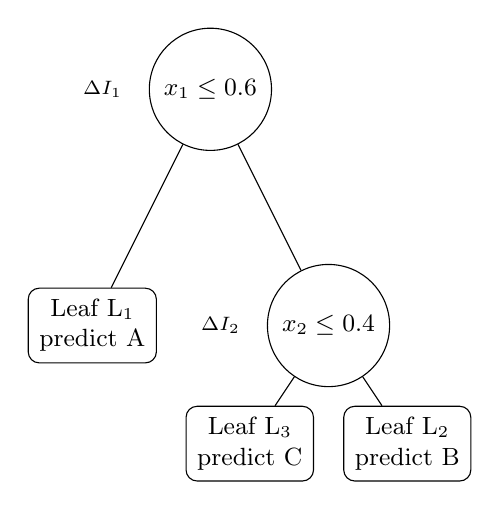
\begin{tikzpicture}[
    every node/.style={font=\small},
    leaf/.style={rectangle,draw,rounded corners,inner sep=4pt},
    split/.style={circle,draw,inner sep=4pt}
]
    % Root node
    \node[split] (root) at (0,2) {$x_1 \le 0.6$};
    
    % Left child (leaf)
    \node[leaf,align=center] (L1) at (-1.5,-1) {Leaf L$_1$ \\ predict A};
    \draw (root) -- (L1);
    
    % Right child (split node)
    \node[split] (r) at (1.5,-1) {$x_2 \le 0.4$};
    \draw (root) -- (r);
    
    % Right child's children (leaves)
    \node[leaf,align=center] (L3) at (0.5,-2.5) {Leaf L$_3$ \\ predict C};
    \node[leaf,align=center] (L2) at (2.5,-2.5) {Leaf L$_2$ \\ predict B};
    \draw (r) -- (L3);
    \draw (r) -- (L2);
    
    % impurity reductions (optional annotations)
    \node[font=\scriptsize,anchor=east] at ([xshift=-1.0cm]root) {$\Delta I_1$};
    \node[font=\scriptsize,anchor=east] at ([xshift=-1.0cm]r) {$\Delta I_2$};
\end{tikzpicture}

\end{document}
